\documentclass[12pt,a4paper]{article}
\synctex=1
\usepackage[utf8]{inputenc}
\usepackage[margin=1cm]{geometry}
\usepackage{graphicx}
%\usepackage{verbatim}
\usepackage{listings}
\usepackage{textcomp}
\usepackage{courier}
\usepackage{libertine}
\usepackage{pgfornament}
\usepackage{eso-pic}
\usepackage[hangul]{kotex}
\linespread{1.3}

\title{
	\centering
	\pgfornament[width=12cm,color=teal]{84}\\
	\vspace{1cm}
	\fontsize{50}{50} \selectfont {컴퓨터 그래픽스 입문}\\
		\pgfornament[width=12cm,color=teal]{88}\\
	\vfill}
\author{
	\LARGE
	\begin{tabular}{rl}
		\hline
		학번 : & 2016110056\\ 
		학과 : & 불교학부 \\
		이름 : & 박승원\\
		날짜 : & \today\\
		\hline
	\end{tabular}\vspace{2cm}
	\\

\includegraphics[width=0.5\textwidth]{logo.jpg}
	}
\date{}


\begin{document}
\maketitle
\pagenumbering{gobble}
\noindent
\lstset{language=C++, columns=flexible, tabsize=4, frame=shadowbox, showstringspaces=false, breaklines=true, upquote=true, basicstyle=\normalsize}
\newpage
\section*{Lab 6. Modeling}

Programming Practice
\subsection{Transform your ironman model to make it look correctly. (5pt)}
\lstinputlisting[caption=obj파일 리더 헤더파일]{src/readobj.h}
\lstinputlisting[caption=obj파일 리더 구현부]{src/readobj.cc}
\lstinputlisting[caption=실행파일]{src/val2.cpp}
대부분의 모듈은 이미 지난 시간에 제출한 것을 재활용해서 다시 올리지 않습니다.

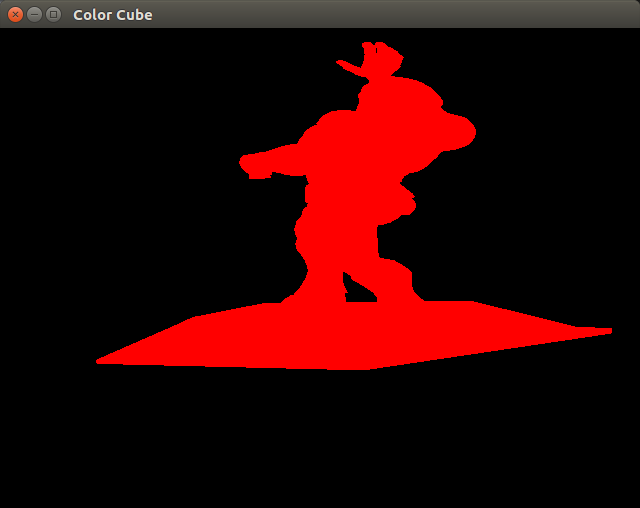
\includegraphics[width=\textwidth]{3.png}
파일명을 인자로 해서 obj 파일을 읽어들이는 방식으로 했다.\\
scale만을 조절해서 아이언맨을 표시할 수 있었다.
\subsection{Use Blender (or other modeling software) to model a simple (and probably cute) 3D smiley. Export it to an OBJ file and read it in YOUR program. (5pt)}
\lstinputlisting[caption=위의 실행 파일에서 눈을 검게 하고 구를 노란색으로 하기 위해 한 줄만을 첨가했다.]{src/val3.cpp}
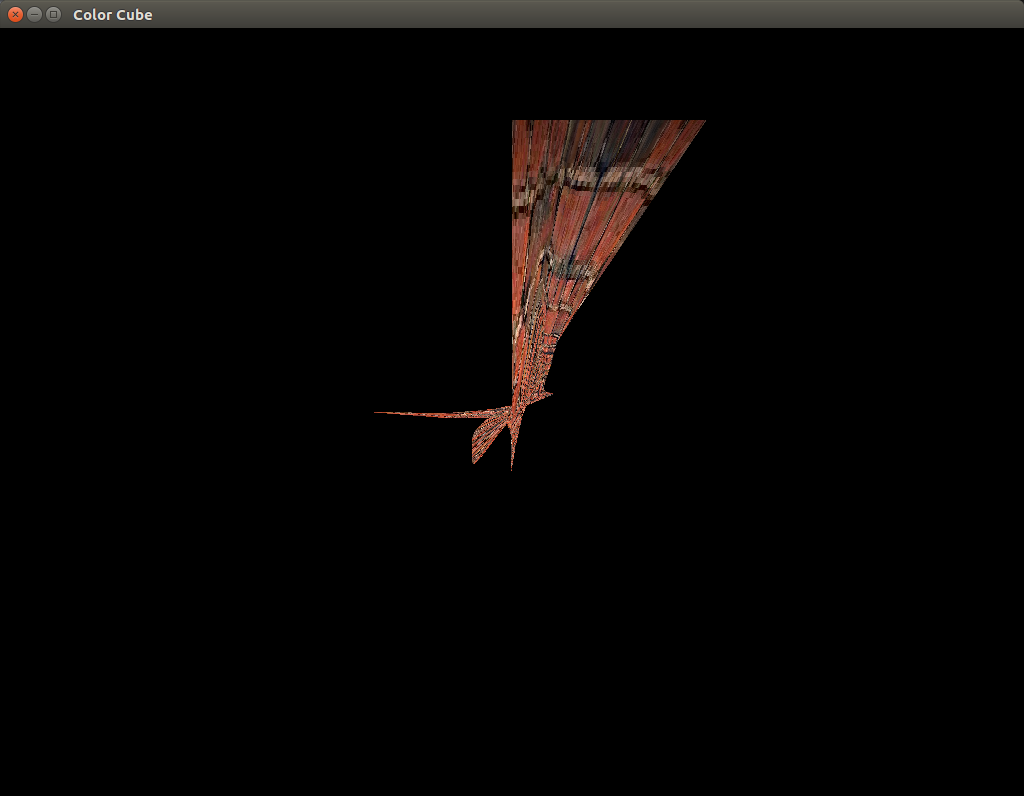
\includegraphics[width=\textwidth]{1.png}

입이 있다는 것을 표현하기 위해 옆으로 돌린 모습.\\
블렌더가 익숙하지 않아 예쁜 모양은 나오지 않았지만, 얼굴을 구로 눈을 디스크로 입을 토루스로 표현해보았다.\\
입의 색깔이 같은 색이라 정면에서는 보이지 않아 옆으로 돌려보았다.

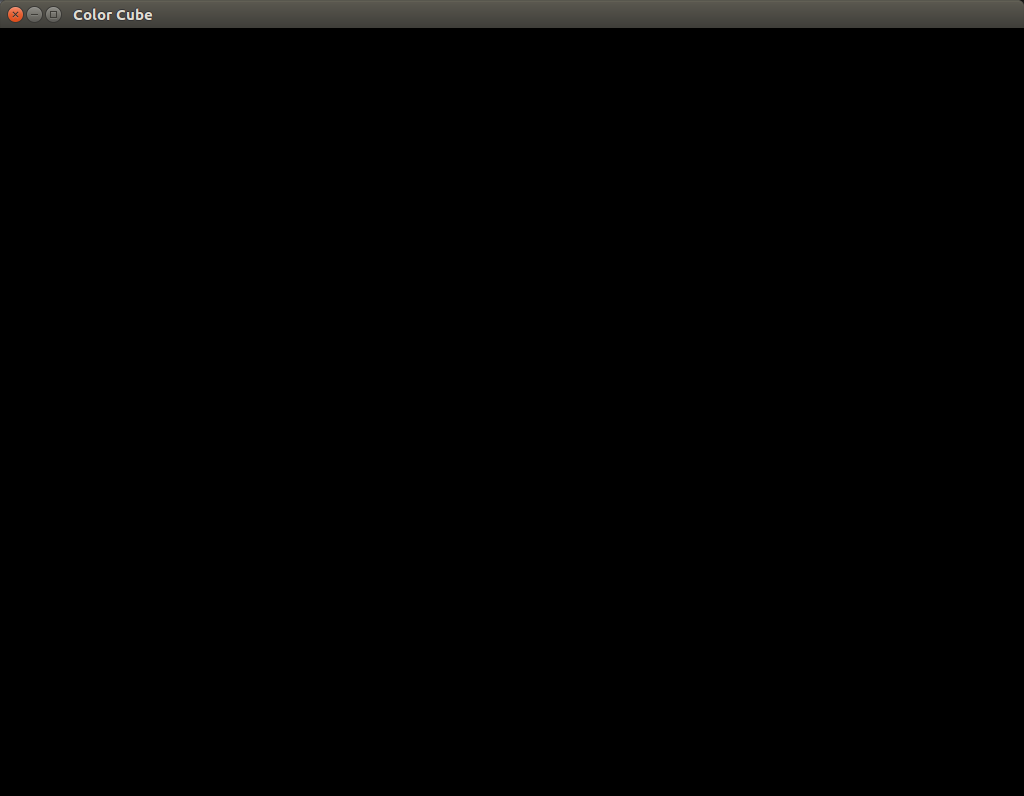
\includegraphics[width=\textwidth]{2.png}

정면에서 본 모습\\삼각형으로 만들어 obj를 구현하는 데에는 성공했다.\\
Ugly!! 죄송합니다...

\end{document}
